\documentclass{article}
\usepackage[utf8]{inputenc}

\usepackage{float}
\restylefloat{table}

\usepackage{graphicx}
\usepackage{color}

\usepackage{geometry}
\geometry{hmargin=2.5cm,vmargin=1.5cm}

\begin{document}

\begin{figure}[t]
\centering

\includegraphics[width=5cm]{inp_n7.png}
\end{figure}

\title{\vspace{4cm} \textbf{Étude de chaînes de transmission sur fréquence porteuse}}
\author{Nom des auteurs\\ \textsc{Cazes} Noa\\ \textsc{Martin} Cédric}
\date{\vspace{11cm} Département Sciences du Numérique - Première année \\
2019-2020 }

\maketitle

\newpage
\tableofcontents
\listoffigures

\newpage


\section{Introduction}

\setlength\parindent{0.5cm}
Après avoir étudié les chaînes de transmisssion en bande de base, notre étude se porte ici sur les chaînes de transmission sur fréquence porteuse. Il n'est plus alors question d'étuder l'impact des filtres de réception ou de mise en forme sur l'efficacité spectrale et en puissance, mais plutôt de comparer chaîne sur fréquence porteuse et sa chaîne passe-bas équivalente, puis de comparer l'impact du mapping sur l'efficacité spectrale et en puissance.  


\section{Utilisation de la chaine passe-bas équivalente pour le calcul et l'estimation du taux d'erreur binaire}

L'objectif de cette partie est de montrer que le taux d'erreur binaire obtenu pour une transmission est identique que l'on implante la chaine de transmission sur fréquence porteuse ou bien la chaine passe-bas équivalente. L'étude sera réalisée pour une transmission QPSK.

\subsection{Etude théorique}
On considère la chaine de transmission passe-bas équivalente à une chaine de transmission QPSK (symboles $d_k \in \left\{\pm 1 \pm j\right\}$), avec filtre de mise en forme et filtre de réception en racine de cosinus surélevé de même roll off et un canal à bruit additif blanc et Gaussien. La figure \ref{rcf} donne le tracé de la réponse en fréquence globale de la chaine de transmission : $G(f)=H(f)H_r(f)$, où $H(f)$ représente la réponse en fréquence du filtre de mise en forme et $H_r(f)$ la réponse en fréquence du filtre de réception.

\begin{figure*}[h!]
\begin{center}
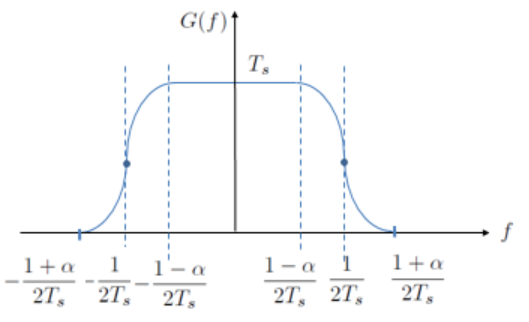
\includegraphics[width=7cm]{RCF.PNG}
\end{center}
\caption{Réponse en fréquence de la chaine de transmission} \label{rcf}
\end{figure*}

\begin{enumerate}
    \item Calculer l'énergie symbole $E_s$ à l'entrée du récepteur. Attention $E_s$ représente la véritable énergie reçue, c'est-à-dire qu'elle doit être calculée à partir de la véritable puissance du signal reçu, pas à partir de celle de l'enveloppe complexe associée.
   
        
    \item Calculer la puissance du bruit sur chaque voie (I et Q) en sortie du filtre de réception.
    \item Les deux voies I et Q étant indépendantes, donner le taux d'erreur symbole de la modulation QPSK en fonction de ceux des voies I et Q ($TES_I$ et $TES_Q$).
    \item En suppposant les termes du deuxième ordre négligeables ($TES_I \times TES_Q \sim 0$) , donner le taux d'erreur symbole de la modulation QPSK en fonction de $TES_I$ uniquement.
    \item Déterminer $TES_I$ en fonction de $\frac{E_s}{N_0}$, $E_s$ correspondant à la véritable énergie reçue. On supposera que les instants d'échantillonnage et l'organe de décision sont optimaux.
    \item En déduire le taux d'erreur binaire de la chaine de transmission QPSK en fonction de $\frac{E_b}{N_0}$.
\end{enumerate}

\subsection{Implantation sous Matlab}
\subsubsection{Implantation de la chaine sur fréquence porteuse}
\begin{enumerate}
    \item Tracer les signaux générés sur les voies en phase et en quadrature ainsi que le signal transmis sur fréquence porteuse.
    \item Estimer par périodogramme puis tracer la densité spectrale de puissance du signal modulé sur fréquence porteuse. Le tracé observé (forme, position) correspond-il à ce qui est attendu en théorie ? Expliquez votre réponse.
    \item Implanter la chaine complète sans bruit afin de vérifier que le TEB obtenu est bien nul.
    \item Rajouter le bruit et tracer le taux d'erreur binaire obtenu en fonction du rapport signal à bruit par bit à l'entrée du récepteur ($E_b/N_0$) en décibels. On prendra des valeurs de $\left(E_b/N_0\right)_{dB}$ allant de $0$ à $6$ dB.
    \item Comparer le TEB simulé au TEB théorique de la chaine étudiée (tracé superposés sur une même figure). Ce tracé doit permettre de valider le bon fonctionnement de votre chaine de transmission.
\end{enumerate}

\subsubsection{Implantation de la chaine passe-bas équivalente}
\begin{enumerate}
    \item Tracer les signaux générés sur les voies en phase et en quadrature.
    \item Estimer par périodogramme puis tracer la densité spectrale de puissance de l'enveloppe complexe associée au signal modulé sur fréquence porteuse. Le tracé observé (forme, position) correspond-il à ce qui est attendu en théorie ? Expliquez votre réponse. On comparera notament ce tracé avec celui obtenu pour la DSP du signal sur fréquence porteuse précédemment.
    \item Implanter la chaine complète sans bruit afin de vérifier que le TEB obtenu est bien nul.
    \item Rajouter le bruit et tracer le taux d'erreur binaire obtenu en fonction du rapport signal à bruit par bit à l'entrée du récepteur ($E_b/N_0$) en décibels. On prendra des valeurs de $\left(E_b/N_0\right)_{dB}$ allant de $0$ à $6$ dB.
    \item Tracer les constellations en sortie du mapping et en sortie de l'échantillonneur pour une valeur donnée de $E_b/N_0$.
    \item Vérifier que l'on obtient bien le même TEB que celui obtenu avec la chaine simulée sur fréquence porteuse (tracé sur une même figure).
\end{enumerate}

%%%%%%%%%%%%%%%%%%%%%%%%%%%%%%%%%%%%%%%%%%%%%%%%%%%%%%%%%%%%%%%%%%
\section{Comparaison de modulations sur fréquence porteuse}
%%%%%%%%%%%%%%%%%%%%%%%%%%%%%%%%%%%%%%%%%%%%%%%%%%%%%%%%%%%%%%%%%%

\subsection{Etude théorique}
On considère les quatre chaines de transmission définies dans le tableau suivant ("SRRCF" signifie "Square Root Raised Cosine Filter" ou filtre en racine de cosinus surélevé en français) :

\begin{table} [H]
\begin{center}
  \begin{tabular}{ |c || c | c | c | c |}
    \hline
    Modulation : & $4$-ASK & QPSK & $8$-PSK & $16$-QAM \\ \hline
    Filtre d'emission : & SRRCF, $\alpha=0,5$ & SRRCF, $\alpha=0,5$ & SRRCF, $\alpha=0,5$ & SRRCF, $\alpha=0,5$ \\ \hline
    Filtre de reception : & SRRCF, $\alpha=0,5$ & SRRCF, $\alpha=0,5$ & SRRCF, $\alpha=0,5$ & SRRCF, $\alpha=0,5$ \\ \hline
    Debit binaire : & $48$ kbps & $48$ kbps & $48$ kbps & $48$ kbps \\ \hline
    TEB :  & $10^{-2}$ & $10^{-2}$ & $10^{-2}$ & $10^{-2}$ \\ \hline
    \hline

  \end{tabular}
\end{center}
% \caption{Comparaison de trois systemes de transmission.}
  \label{table:minus6db}
\end{table}

\begin{enumerate}
    \item Tracer les constellations des quatre modulations considérées.
    \item Déterminer le débit symbole ($R_s$) dans les quatre cas.
    \item Calculer les efficacités spectrales des quatre transmissions proposées. Quelle est la transmission la plus efficace spectralement ? Qu'est-ce que cela veut dire ?
    \item La figure \ref{comp_TEB} donne les courbes de  TEB obtenus en fonction du rapport signal à bruit par bit à l'entrée du récepteur ($E_b/N_0$) en dB, pour les quatre transmissions considérées réalisées sur canal à bruit additif et Gaussien.
        \begin{itemize}
            \item En déduire les valeurs de $E_b/N_0$ nécessaires pour satisfaire à la spécification du TEB. Quel est le système le plus efficace en terme de puissance ? Justifiez votre réponse.
            \item La chaine de transmission utilisant la modulation $4$-ASK et la chaine de transmission utilisant la modulation $16$-QAM présentent le même taux d'erreur binaire. Qu'est-ce-qui pourrait justifier le choix de l'une ou l'autre ?
        \end{itemize}
    \item Si on souhaitait réaliser la transmission à travers un canal de propagation supposé à bruit additif blanc et Gaussien (AWGN) de bande passante $20$ kHz, serait-il possible de réaliser chaque transmission proposée en trouvant, au niveau du récepteur, un instant optimal d'échantillonnage sans interférence entre symboles ? Expliquez votre réponse.
\end{enumerate}

 \begin{figure}[ht!]
    \centering
    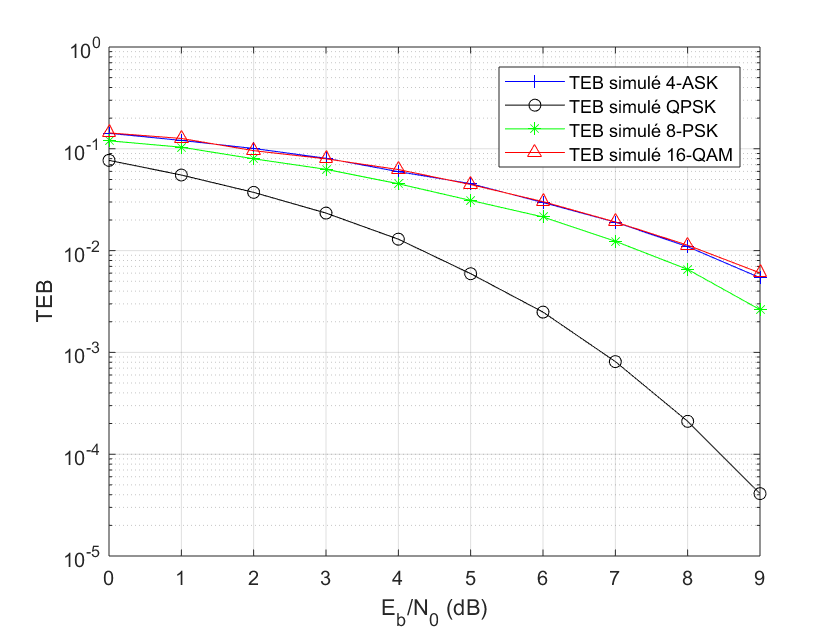
\includegraphics[width=12cm]{Comp_TEB.png}
    \caption{Comparaison des TEB pour les modulations ASK, PSK et QAM}
    \label{comp_TEB}
 \end{figure}

\subsection{Implantation sous Matlab}
Il s'agira d'implanter, d'analyser et de comparer les chaines passe-bas équivalentes associées aux chaines de transmissions proposées dans l'étude théorique.
Pour cela :
\subsubsection{Etude de chaque chaine de transmission}
\begin{enumerate}
    \item Implanter la chaine complète sans bruit afin de vérifier que le TEB obtenu est bien nul. On pourra utiliser les fonctions Matlab \emph{pskmod.m}, \emph{pskdemod.m }et \emph{qammod.m}, \emph{qamdemod.m} pour réaliser les mapping/demapping et prises de décision.
    \item Rajouter le bruit et :
        \begin{itemize}
            \item Tracer les constellations en sortie du mapping et en sortie de l'échantillonneur pour différentes valeurs de $E_b/N_0$, en expliquant les différences observées.
            \item Tracer le taux d'erreur binaire obtenu en fonction du rapport signal à bruit par bit à l'entrée du récepteur ($E_b/N_0$) en décibels. On prendra des valeurs de $\left(E_b/N_0\right)_{dB}$ allant de $0$ à $6$ dB.
            \item Comparer le TEB simulé au TEB théorique de la chaine étudiée (tracé superposés sur une même figure). Ce tracé doit permettre de valider le bon fonctionnement de votre chaine de transmission. Les TEBs théoriques sont donnés dans les planches de cours.
        \end{itemize}
\end{enumerate}

\subsubsection{Comparaison des chaines de transmission}
\begin{enumerate}
    \item En utilisant les tracés obtenus pour leurs TEBs, comparer et classer les différentes chaines de transmission en en termes d'efficacité en puissance (en expliquant votre raisonnement).
    \item Pour un même débit binaire, tracer les densités spectrales de puissance des signaux émis dans les différentes chaines de transmission étudiées afin de les comparer en termes d'efficacité spectrale et de les classer (en expliquant votre raisonnement).\\
\end{enumerate}

\section{Conclusion}
\textcolor{blue}{A compléter}

\section{Références}
\textcolor{blue}{A compléter}


\end{document}
